\documentclass[../main]{subfiles}

\graphicspath{{../figures/}}

\begin{document}

\section{プラント内音響点検の特徴と課題}
\label{sec:intro_anomaly-detection}
\refsec{sec:intro_background}で述べたように石油精製プラント内には多くの異常が存在し,
高齢化や熟練度の差による点検品質のばらつきといった様々な課題を解決するため,
プラント内点検の自動化が求められている.
プラント内音響点検には自動化にあたって以下のような特徴と課題がある.


まず,プラント内音響点検の課題としてプラント内で異常音を取得するのが難しいことがあげられる.
プラント内に存在する機器から異常音が出るのは機器が故障した時であり,機器の故障が起こる頻度は少ないため,
異常音が発生する頻度はかなり少ない.
また,機器の故障が起こる際は時間の経過とともに徐々に壊れていくことが多いため,異常音と明確に判断されたデータを収集することは非常に困難である.
更に,ベアリングのような機器は傷の種類や深さによって異常音の特徴が多岐にわたり,そのような多様な異常音のデータを収集することも同様に困難である.
そのため,正常音のみを用いて異常を検出する必要がある.

次にプラント内では音源となる機器が密集していることがあげられる.
\reffig{fig:pump_location}に示すように,プラント内には稼働中に音を発する様々な機器が密集して存在しており,
これらの機器から発せられる音はそれぞれが非常に大きく,
異常の有無のみではなく,異常音源の位置特定が重要である.

このようにプラント内環境で異常音を検知するためには,プラント特有の様々な課題が存在する.
本研究では,マイクロホンを搭載した移動ロボットを用いてプラント内環境特有の
異常音検知における課題を解決する手法を提案する.

\begin{figure}[t]
  \centering
  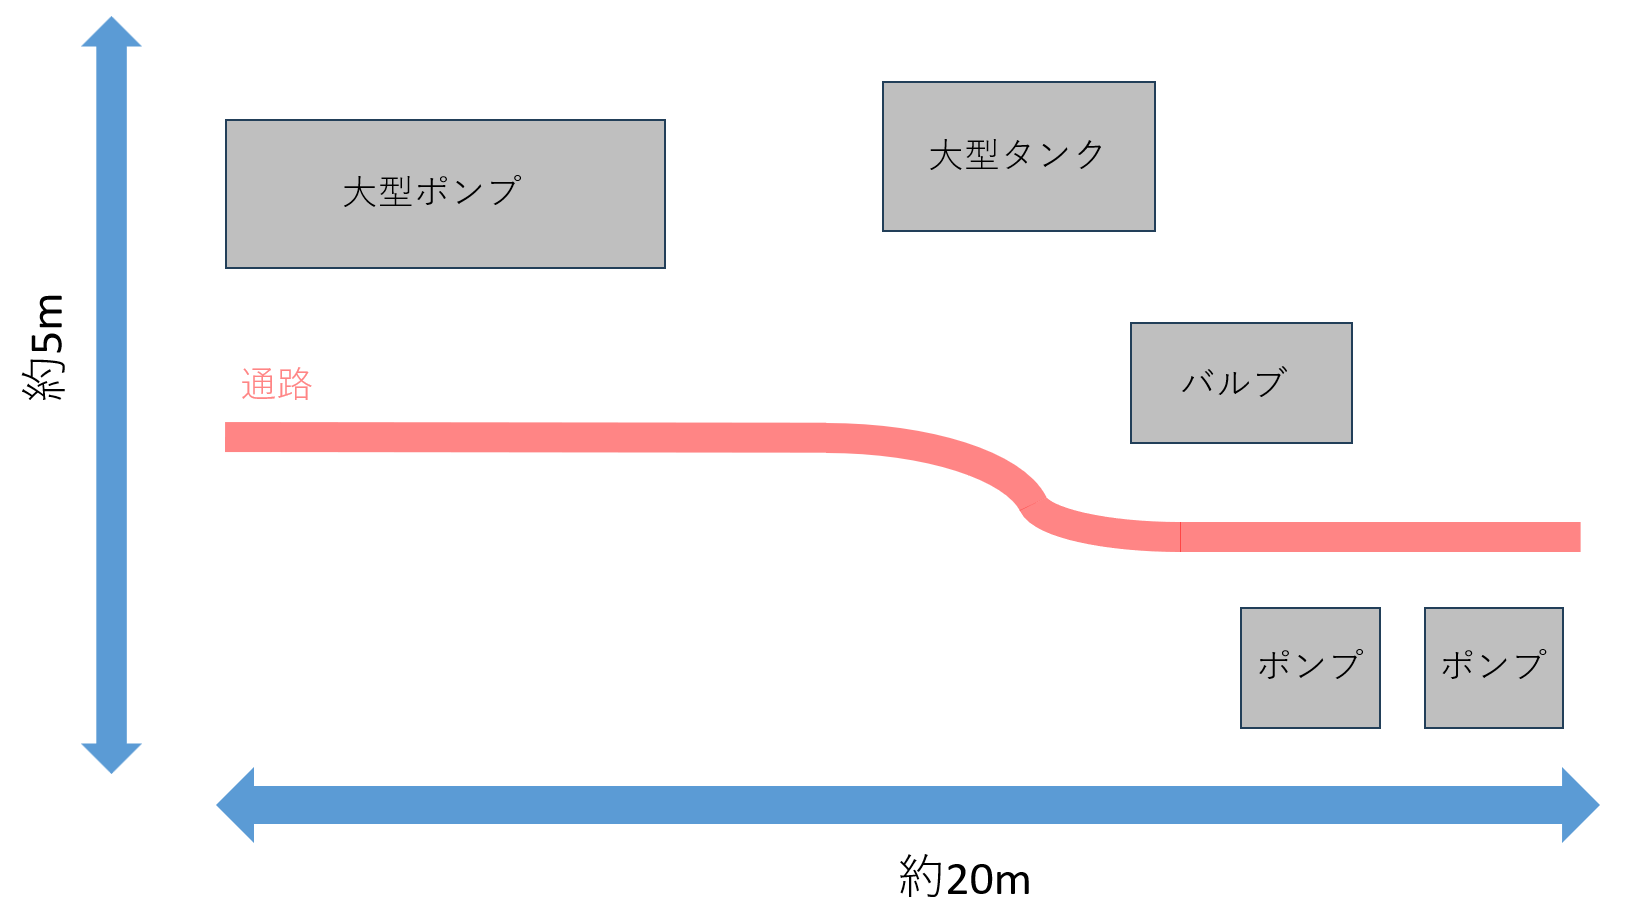
\includegraphics[keepaspectratio, width=1.0\linewidth]{chap1/pump_location.png}
  \caption{石油精製プラントのポンプ配置図の1例}
  \label{fig:pump_location}
\end{figure}

\end{document}
